\documentclass[11pt,a4paper]{article}
\usepackage{fontspec}
\setmainfont{TeX Gyre Pagella}
\newfontfamily\headfont{Inter}[UprightFont=*-ExtraBold,BoldFont=*-ExtraBold,Extension=.otf,Path=/usr/share/fonts/opentype/inter/]
\usepackage[a4paper,margin=2.3cm]{geometry}
\usepackage{graphicx,booktabs,float,caption,array,xcolor,longtable}
\usepackage{xurl}
\usepackage[hidelinks]{hyperref}
\usepackage{titlesec}
\usepackage[round]{natbib}
\usepackage{setspace}
\setstretch{1.05}
\renewcommand{\topfraction}{0.9}
\renewcommand{\bottomfraction}{0.8}
\renewcommand{\textfraction}{0.1}
\renewcommand{\floatpagefraction}{0.75}
\setlength{\parindent}{0pt}
\setlength{\parskip}{0.55em}
\titleformat{\section}{\headfont\Large}{\thesection}{0.8em}{}
\titleformat{\subsection}{\headfont\large}{\thesubsection}{0.8em}{}
\captionsetup{font=small,labelfont=bf}
\urlstyle{same}
\hypersetup{pdftitle={The Wealth of Nations, Mapped},pdfauthor={Tristan Hotham}}

\begin{document}
\begin{center}
{\Large\bfseries The Wealth of Nations, Mapped\par}
\vspace{0.4em}
{\large National output, output per head and shares of the world economy\\on an interactive map, with world estimates from 10,000 BC\par}
\vspace{1.2em}
{\large Tristan Hotham\par}
\vspace{0.3em}
{\small Independent researcher\\
ORCID: 0000-0003-4931-9349\\
DOI: https://doi.org/10.5281/zenodo.23899403\par}
\vspace{0.8em}
2026
\end{center}

\begin{quote}
\small
\begin{center}\textbf{Abstract}\end{center}
I put the Maddison Project Database 2023 \citep{mpd2023} on an interactive world map with a timeline from AD 1 to 2024, showing for each present-day territory its GDP, GDP per head, share of world GDP and growth, with a ranking of the largest economies, a series for every country and an explicit treatment of the years without estimates. The database holds 21,366 country-year estimates of GDP per head for 169 units, but only 4,387 of them fall before 1820, for 35 countries; I carry the series from 2022 to 2024 with IMF growth rates. In 1820 China and India produced 45.2\% of world output; their share fell to 8.3\% in 1973 and recovered to 30.2\% in 2024, while Western Europe and its offshoots rose from 27.4\% to a peak of 59.2\% in 1913 and fell back to 30.2\%. The United States economy passed Britain's in 1862 and China's by 1887, and was passed by China in purchasing power terms in 2014. Japan's GDP per head grew 6.0-fold between 1950 and 1973 and South Korea's 28-fold between 1960 and 2024. The ratio of the richest to the poorest country's GDP per head (countries of a million people or more) rose from 5.2 in 1820 to 29.5 in 1950 and 251 in 2024; the ratio of the 90th to the 10th percentile country rose from 3.0 to a high near 28 around 2000. Before AD 1 only world totals exist, and they rest largely on assumptions: world population in 3000 BC ranges from 7.8 to 81 million in HYDE 3.2.1, and De Long's world GDP per head barely doubles (2.1 times) between 10,000 BC and 1800, against 15.5 times since 1820. All national values describe present-day territories, and coverage before 1950 is partial.

\textbf{Keywords:} economic history; Maddison Project; GDP per capita; great divergence; historical national accounts; data visualisation; open data
\end{quote}

\section{Introduction}
Angus Maddison's estimates of the size of the world's economies over two millennia \citep{maddison2001,maddison2007} are among the most used, and most argued over, datasets in economic history. Since his death in 2010 the Maddison Project has revised and extended them, replacing many of his own conjectures with new historical national accounts and dropping others; the 2023 release \citep{mpd2023} is the latest. The numbers are usually shown as line charts for a few countries or regions. This paper describes a different view: a world map with a slider, on which every country with an estimate in a given year is coloured, every country without one is hatched, and the largest economies are ranked beside the map. The interactive version is at \url{https://maps.tristanhotham.com/gdp-through-time/}.

The aim is twofold. The map makes the familiar story of the last two centuries, the great divergence between Europe and Asia \citep{pomeranz2000} and the partial convergence since, visible in one place. It also makes the limits of the evidence visible: before 1820, and for much of Africa and Asia before 1950, most of the map is empty. Section~\ref{sec:data} describes the data and the extension to 2024, section~\ref{sec:methods} the derived measures and the map, section~\ref{sec:results} the main findings, and section~\ref{sec:limits} the limitations.

\section{Data}\label{sec:data}
\textbf{Maddison Project Database 2023.} The database gives, for 169 units, real GDP per head in 2011 international dollars (purchasing power parity) and population, from AD 1 to 2022 \citep{mpd2023}. The units are present-day countries, plus three former states (the USSR, Yugoslavia and Czechoslovakia) whose series run alongside those of their successors. Values describe territories within present-day borders: ``Germany'' in 1820 is the territory of modern Germany, ``India'' is the modern Republic of India. Table~\ref{tab:cov} shows how coverage grows. There are estimates of GDP per head for 14 countries in AD 1, all in or beside the Roman world and several sharing one regional figure from \citet{scheidel2009}; 6 in 1000; 11 in 1500; 17 in 1700; 55 in 1820; 75 in 1913; and 146 in 1950. Long annual series before 1820 exist for Britain, France, Spain, Sweden, the Netherlands, Poland, Germany and Portugal, colonial Mexico and Peru, and the Cape (South Africa from 1700); China, Japan and India have estimates at intervals \citep{broadberry2015,broadberry2018,bassino2019,broadberry2015india}. Figure~\ref{fig:cov} shows the number of countries with an estimate in every year.

The database also gives world GDP per head and population at benchmark years (1820, 1850, 1870, 1900, 1920, 1940, each decade from 1950 to 2010, and each year from 2015), computed by its authors from all available estimates; there is no world total before 1820 in this release.

\textbf{The 2011 dollars and their meaning.} GDP per head is converted at 2011 purchasing power parities and extrapolated backwards with the volume growth of each country's own historical national accounts. Comparisons across countries in the distant past therefore rest on long chains of growth rates and on one set of relative prices, and differences of 10 to 20 per cent should not be read as meaningful.

\textbf{Extension to 2024.} The database ends in 2022. I carried each series forward with the IMF World Economic Outlook of October 2025 \citep{weo2025}: GDP grows with the IMF's real GDP per head at PPP times population (or with real GDP growth where the per head series is missing), and population with the IMF's population. This covers 166 units; Cuba, North Korea and Syria, which the IMF does not cover, are held at 2022 in world totals and shown only to 2022. For former states the successors' combined growth is used. For some countries the IMF's figures for 2024 are themselves estimates (129 country-years); they are flagged on the map.

\textbf{The very long run.} Before AD 1 there are no national or regional estimates. For the world as a whole I use the estimates of world GDP and GDP per head of \citet{delong1998} (his variant without the Nordhaus adjustment, closest to Maddison's concept) and world population from HYDE 3.2.1 \citep{hyde2017}, with its low and high range, and from \citet{mcevedy1978}. For AD 1, 1000, 1500, 1600 and 1700 I add Maddison's own regional estimates \citep{maddison2010} for 11 regions, which the 2023 database no longer carries. All of these were taken from the transcription by \citet{roodman2020}. They are in 1990 dollars; I rescale them by a single factor (1.694) so that Maddison's 2010 world GDP per head in 1820 equals the 2023 database's. Table~\ref{tab:lr} lists the values.

\begin{table}[tbp]\centering\small\caption{The very long run: world population (million) from HYDE 3.2.1 (central, low to high) and McEvedy and Jones, and world GDP per head (2011 int.\ \$, linked at 1820) from De Long (1998) and Maddison (2010). *De Long 1800.}\label{tab:lr}\begin{tabular}{lrrrrr}\toprule Year & HYDE & HYDE range & McEvedy, Jones & De Long & Maddison 2010\\\midrule
10,000 BC & 4.4 &  & 4 & 583 & \\
5,000 BC & 19.1 & 2.4 to 36 & 5 & 645 & \\
3,000 BC & 44.5 & 7.8 to 81 & 14 &  & \\
2,000 BC & 72.6 & 14.5 to 131 & 27 &  & \\
1,000 BC & 110.4 & 24.8 to 196 & 50 & 798 & \\
AD 1 & 232.1 &  & 170 & 684 & 791\\
1000 & 323.4 & 176.0 to 471 & 265 & 837 & 768\\
1500 & 503.2 & 347.8 to 659 & 425 & 867 & 959\\
1820 & 1,052.8 & 915.9 to 1,190 &  & 1,223* & 1,128\\
\bottomrule\end{tabular}\end{table}

\textbf{Maps.} Present-day borders are Natural Earth 1:50m countries \citep{naturalearth}; 169 Maddison units map onto them, with South Sudan drawn with Sudan (Maddison's ``Sudan (Former)'') and the territories of the USSR, Yugoslavia and Czechoslovakia dissolved into one shape until those states broke up (1991, 1991, 1992). Borders of the time come from the historical-basemaps project \citep{ourednik}, 52 snapshots from AD 1 to 2010, simplified, drawn only as a faint dashed backdrop and used to name the state a clicked point lay in.

\begin{table}[tbp]\centering\small\caption{Coverage at selected years: units with an estimate of GDP per head, with GDP (population known or interpolated), share of world population in units with GDP (\%), and world GDP (trillion 2011 int.\ \$) and GDP per head. Units include former states and their successors.}\label{tab:cov}\begin{tabular}{lrrrrr}\toprule Year & GDP per head & GDP & Population covered & World GDP & World per head\\\midrule
AD 1 & 14 & 12 &  & & \\
1000 & 6 & 6 &  & & \\
1500 & 11 & 11 &  & & \\
1600 & 15 & 15 &  & & \\
1700 & 17 & 17 &  & & \\
1820 & 55 & 55 & 65.5 & 1.2 & 1,128\\
1870 & 70 & 67 & 93.2 & 2.0 & 1,543\\
1913 & 75 & 68 & 93.0 & 4.3 & 2,411\\
1950 & 146 & 146 & 99.6 & 8.5 & 3,360\\
1973 & 167 & 167 &  & 25.5 & 6,536\\
2000 & 169 & 169 &  & 59.9 & 9,904\\
2022 & 169 & 169 &  & 130.1 & 16,677\\
2024 & 166 & 166 &  & 139.2 & 17,511\\
\bottomrule\end{tabular}\end{table}

\begin{figure}[tbp]\centering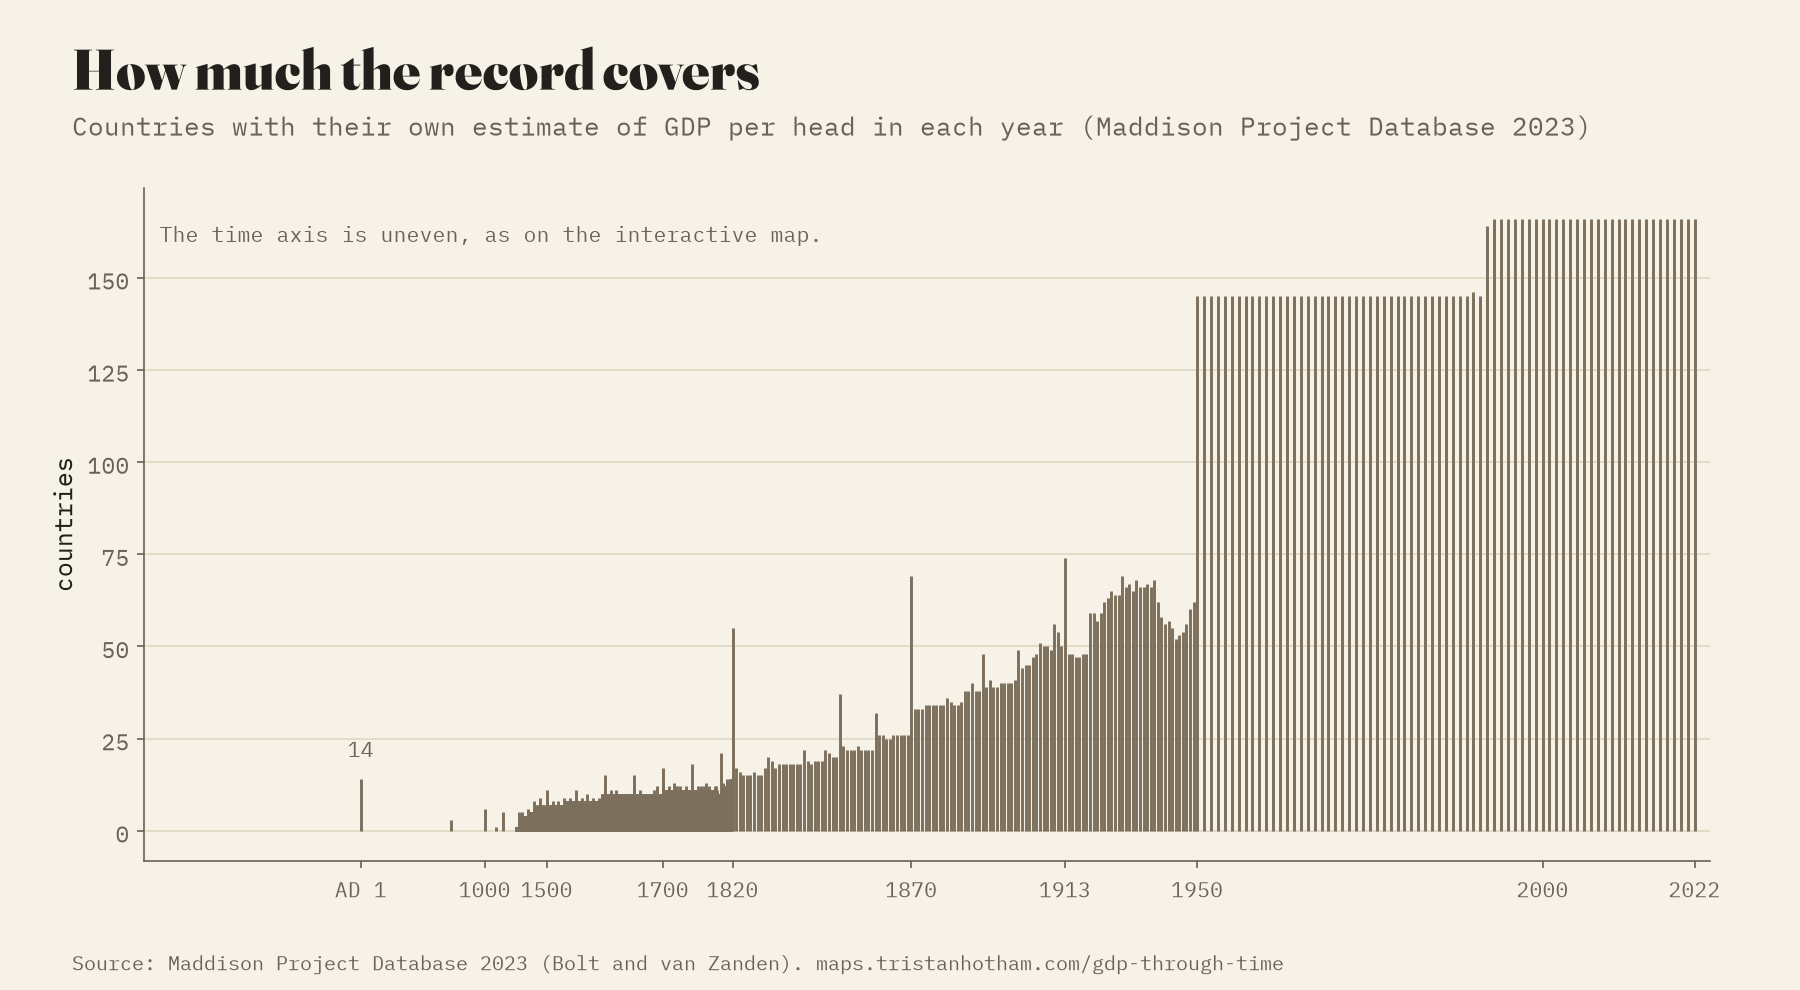
\includegraphics[width=\textwidth]{f_coverage.png}
\caption{Countries with their own estimate of GDP per head in each year, Maddison Project Database 2023 (former states counted until they broke up, their successors after). The time axis is uneven, as on the interactive map.}\label{fig:cov}\end{figure}

\section{Methods}\label{sec:methods}
\textbf{Total GDP.} GDP is GDP per head times population. Where a year has GDP per head but no population, population is interpolated log-linearly between the database's population estimates if they are at most 30 years apart (409 country-years); otherwise the year has GDP per head but no total.

\textbf{World GDP and shares.} At the database's benchmark years world GDP is its world GDP per head times world population. Between benchmarks before 1950 it is interpolated log-linearly. From 1950 the yearly world total is the sum of countries (without double counting former states and their successors), scaled by the ratio of the benchmark world total to that sum, interpolated between benchmarks; the ratio lies between 0.9972 and 1.0043, so the scaling is small. Shares of world GDP are a country's GDP over the world total in the same year. In 1820 the countries with estimates hold 65.5\% of the world's population (the rest is in the database's world total through its regional estimates); in 1870, 93.2\%; in 1950, 99.6\%.

\textbf{Growth.} For each estimate of GDP per head, growth is the annual average change since the country's estimate closest to ten years earlier, if one exists between 5 and 15 years earlier.

\textbf{Gaps and nearest estimates.} On the map a country with no estimate in the chosen year shows its nearest estimate up to 10 years away, dotted (ties go to the earlier year), and is hatched if there is none; readers can switch the filling off. Rankings at benchmark years in this paper use the same rule (so India's 1821 estimate stands for 1820). Overtaking years are judged only on years in which both countries have their own estimate.

\textbf{Former states.} The map shows the USSR, Yugoslavia and Czechoslovakia whole until they broke up and their successors afterwards; world totals use the aggregate when it has an estimate and the successors otherwise.

\section{Results}\label{sec:results}
\subsection{Before the nations}
Figure~\ref{fig:lr} shows world GDP per head and population from 10,000 BC. HYDE's central estimate of world population is 4.4 million in 10,000 BC, 44.5 million in 3000 BC and 232 million in AD 1; McEvedy and Jones give 27 million for 2000 BC, about a third of HYDE's 73 million. De Long's world GDP per head rises from \$583 in 10,000 BC to \$1,223 in 1800 (linked 2011 dollars), a factor of 2.1; it has since risen 15.5 times. The level before AD 1 is close to assumption: De Long anchors it near subsistence and lets population carry most of the growth.

Maddison's regional estimates (Figure~\ref{fig:reg}) give the Indian subcontinent 32.0\% and China 25.4\% of world output in AD 1, and Western Europe, then mostly within the Roman Empire, 13.7\%, falling to 9.0\% in 1000 and rising to 21.8\% in 1700. In AD 1, 7 of the 11 regions have GDP per head of exactly 400, 425 or 450 (1990) dollars, Maddison's assumed values for economies near subsistence, so these shares mostly restate his population estimates. Where his 2010 figures overlap the 2023 database they can differ substantially: China's share in 1820 is 33.0\% in his tables and 28.6\% in the 2023 data.

\begin{figure}[tbp]\centering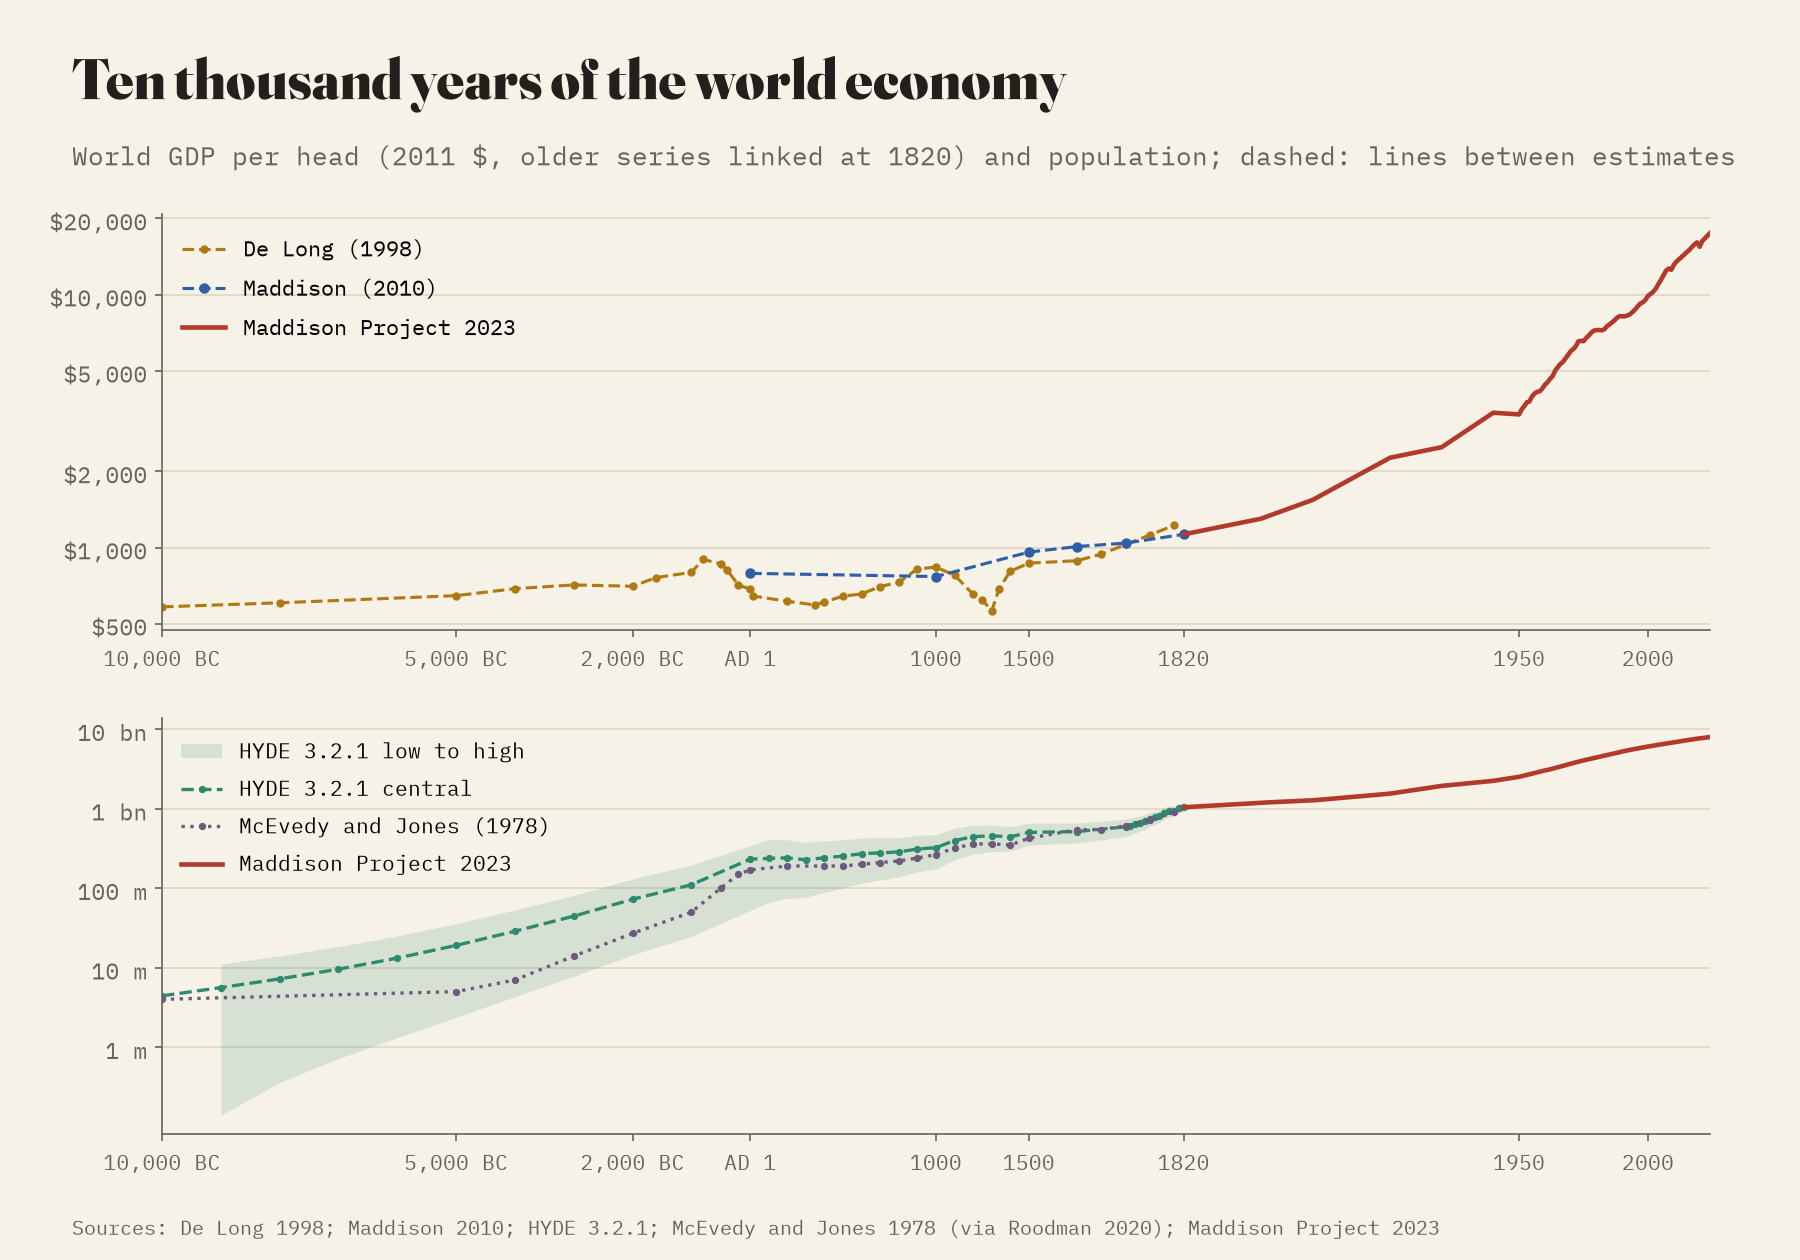
\includegraphics[width=\textwidth]{f_longrun.png}
\caption{World GDP per head and population, 10,000 BC to 2024 (uneven time axis). Dashed lines join estimates that are far apart; the band is HYDE's low to high population range.}\label{fig:lr}\end{figure}

\begin{figure}[tbp]\centering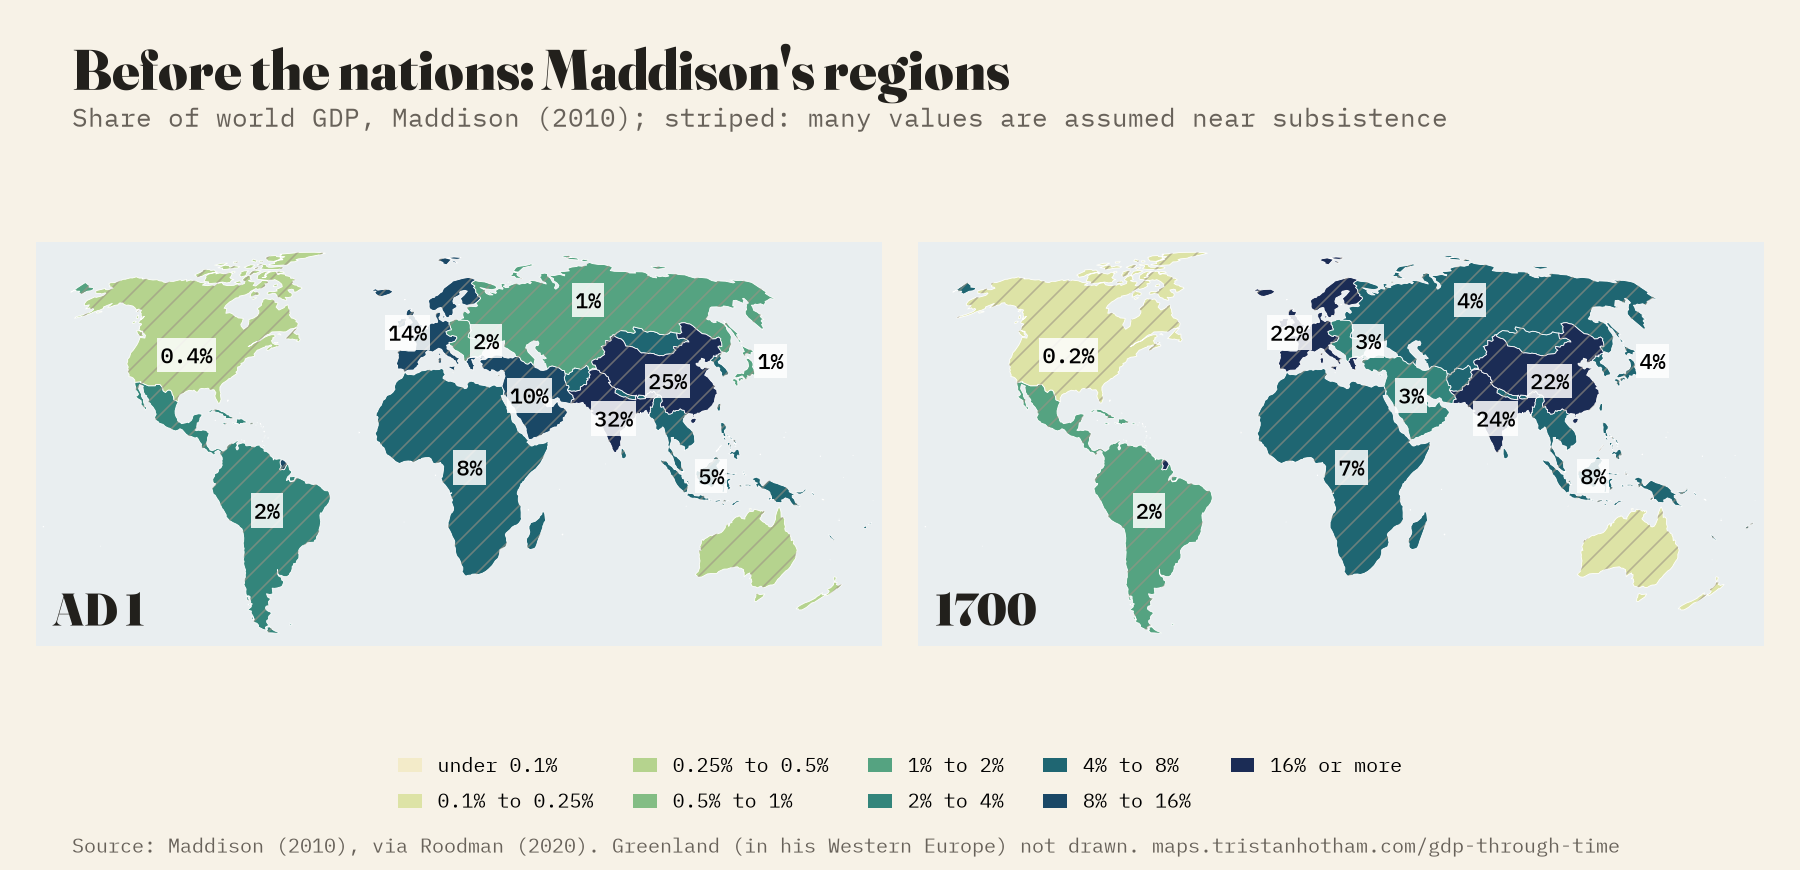
\includegraphics[width=\textwidth]{f_regions.png}
\caption{Maddison's (2010) regional shares of world GDP in AD 1 and 1700.}\label{fig:reg}\end{figure}

\subsection{The divergence and the return}
Figure~\ref{fig:maps} shows each country's share of world GDP in 1820, 1913, 1950 and 2024, and Figure~\ref{fig:share} the shares of the largest economies by year. In 1820 China produced 28.6\% of world output and India (1821) 16.6\%, followed by the United Kingdom (6.0\%), France (4.8\%) and Germany (4.3\%) (Table~\ref{tab:top}). Their size came from population: GDP per head was \$882 in China and \$937 in India, against \$3,306 in the United Kingdom, the richest country of a million people or more.

China's share fell to 10.0\% in 1913, 5.2\% in 1950 and its lowest, 4.2\%, in 1961; India's to 4.2\% in 1950 and 3.0\% in 1979. Together they fell from 45.2\% to 8.3\% in 1973. Western Europe and the Western offshoots rose from 27.4\% in 1820 to 59.2\% in 1913, then declined to 50.7\% in 1973 and 30.2\% in 2024, almost exactly the combined share of China and India (30.2\%). China's share in 2024 is 21.4\% and India's 8.7\%. Because China's estimates before 1950 are a few decades apart (Figure~\ref{fig:share}), the timing of its decline within the nineteenth century is not well determined.

\begin{figure}[tbp]\centering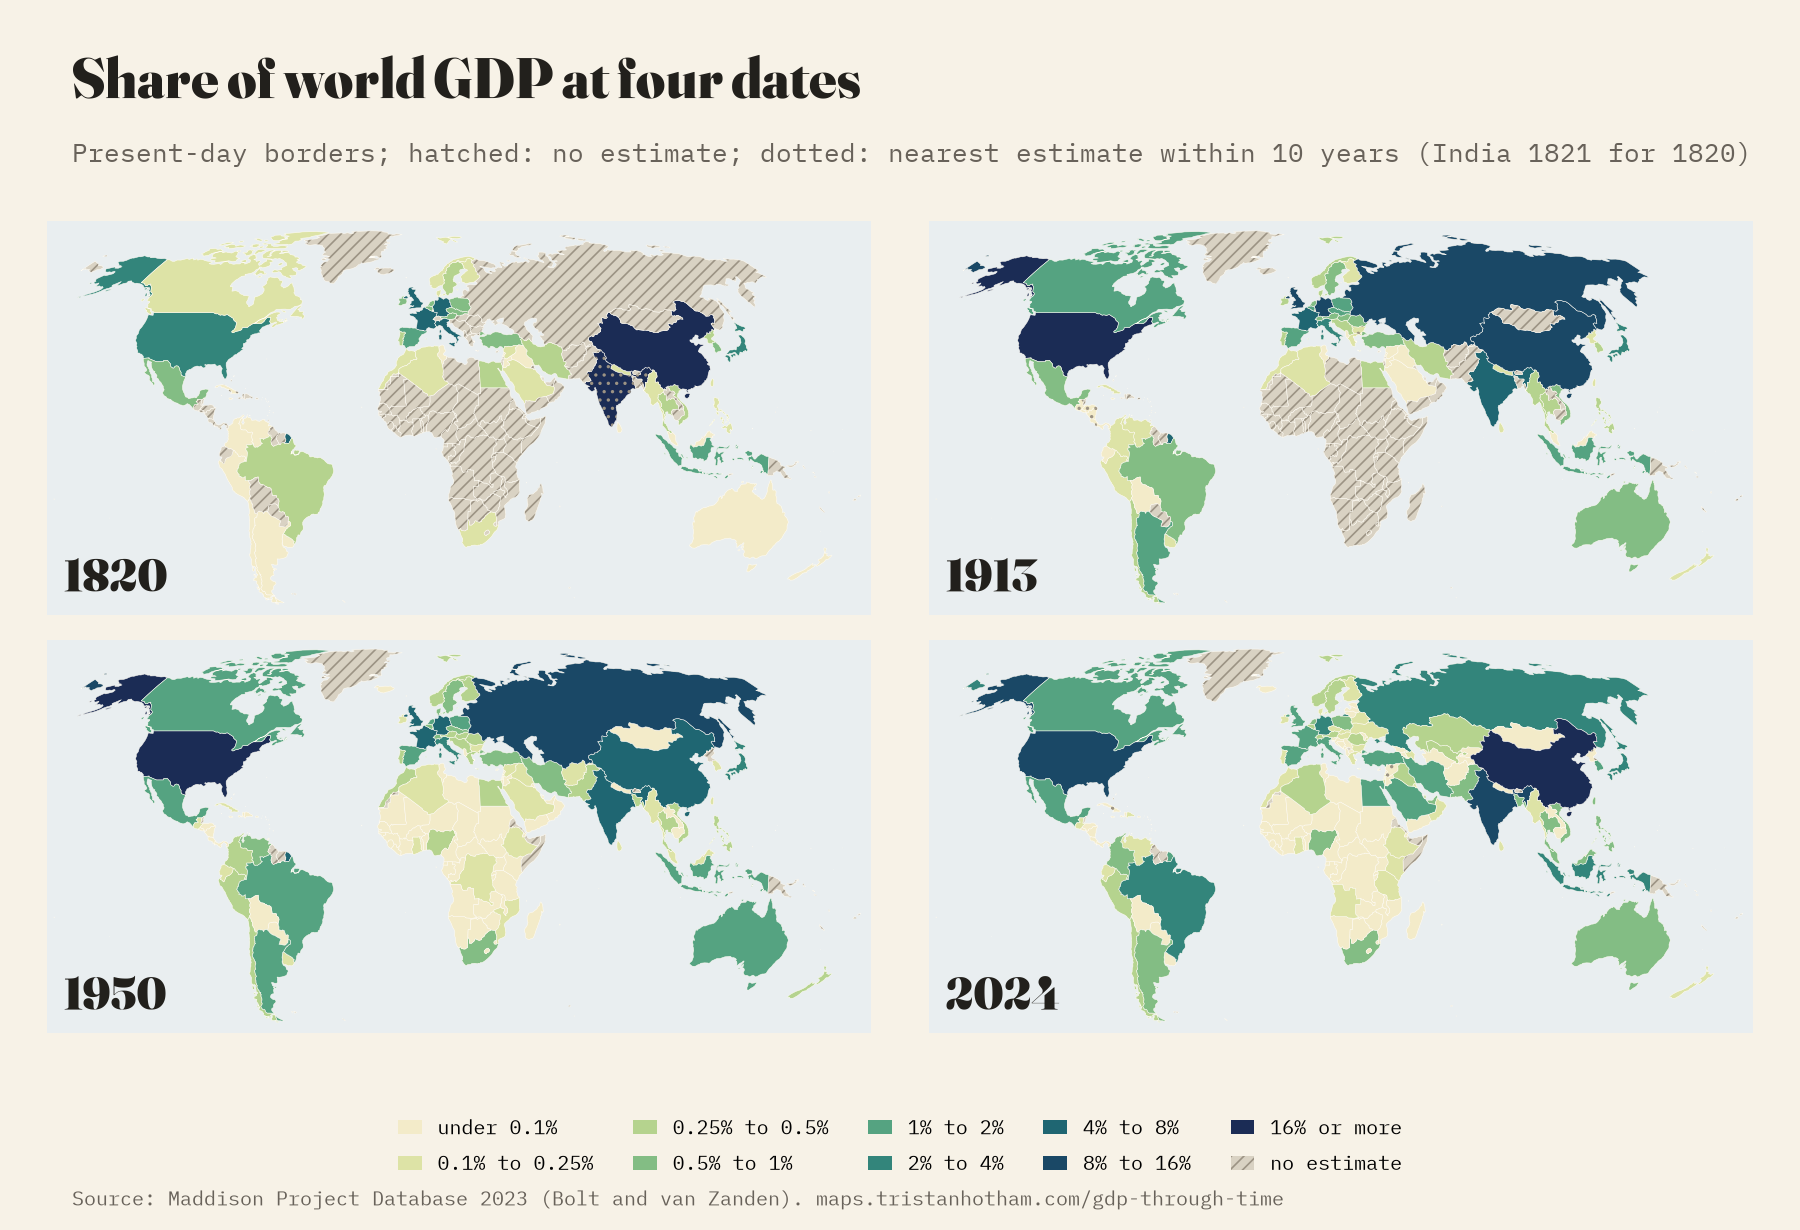
\includegraphics[width=\textwidth]{f_maps.png}
\caption{Share of world GDP at four dates on present-day borders. Hatched: no estimate within ten years; dotted: nearest estimate.}\label{fig:maps}\end{figure}

\begin{figure}[tbp]\centering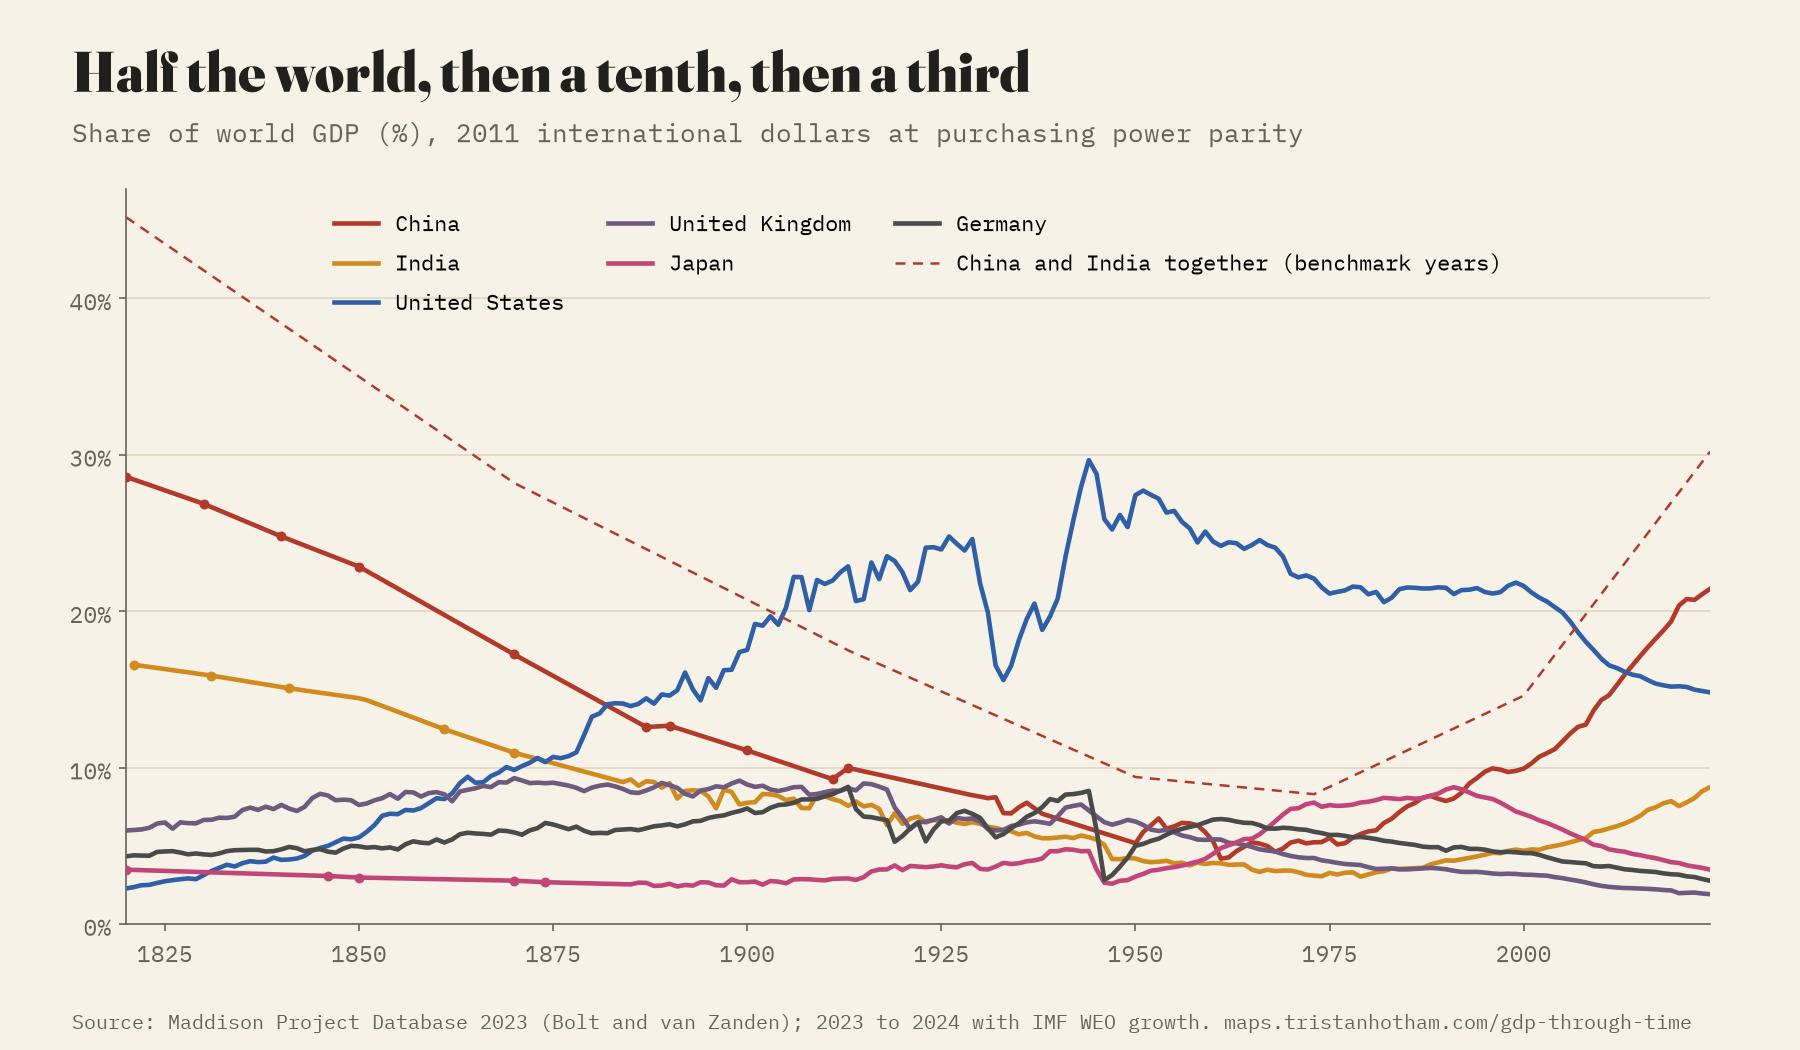
\includegraphics[width=\textwidth]{f_share.png}
\caption{Share of world GDP, 1820 to 2024. Lines join estimates up to 45 years apart; dots mark isolated estimates. The dashed line joins the combined share of China and India at benchmark years.}\label{fig:share}\end{figure}

\begin{table}[tbp]\centering\small\caption{The ten largest economies by share of world GDP (\%) at four dates (nearest estimate within ten years).}\label{tab:top}\begin{tabular}{lrlrlrlr}\toprule \multicolumn{2}{c}{1820} & \multicolumn{2}{c}{1913} & \multicolumn{2}{c}{1950} & \multicolumn{2}{c}{2024}\\\midrule
China & 28.6 & US & 22.9 & US & 27.4 & China & 21.4\\
India & 16.6 & China & 10.0 & USSR & 9.6 & US & 14.8\\
UK & 6.0 & Germany & 8.8 & UK & 6.6 & India & 8.7\\
France & 4.8 & UK & 8.7 & China & 5.2 & Japan & 3.5\\
Italy & 4.3 & USSR & 8.2 & Germany & 5.0 & Russia & 2.9\\
Germany & 4.3 & India & 7.6 & India & 4.2 & Indonesia & 2.8\\
Japan & 3.5 & France & 5.3 & France & 4.2 & Germany & 2.8\\
US & 2.3 & Italy & 3.5 & Italy & 3.1 & Brazil & 2.4\\
Spain & 1.6 & Japan & 2.9 & Japan & 3.0 & France & 2.0\\
Indonesia & 1.3 & Poland & 1.7 & Canada & 1.9 & UK & 1.9\\
\bottomrule\end{tabular}\end{table}

\subsection{Changes of leadership}
The United States economy became larger than the United Kingdom's in 1862 (\$\,149 billion against \$\,140 billion) and stayed larger in every later year. In GDP per head the United States first passed the United Kingdom in 1880, fell behind in some years up to 1898 and in 1933 and 1934, and has been ahead since 1935. The British share of world output peaked at 9.3\% in 1870; the American share at 29.7\% in 1944.

China had the largest GDP in every year with comparable estimates up to 1870. There is no estimate for China between 1870 and 1887; in 1887 the United States was larger. The United States remained the largest economy until 2014, when China passed it in these purchasing power figures, and China has been larger since (Figure~\ref{fig:lead}). Table~\ref{tab:over} lists these and other crossings.

\begin{figure}[tbp]\centering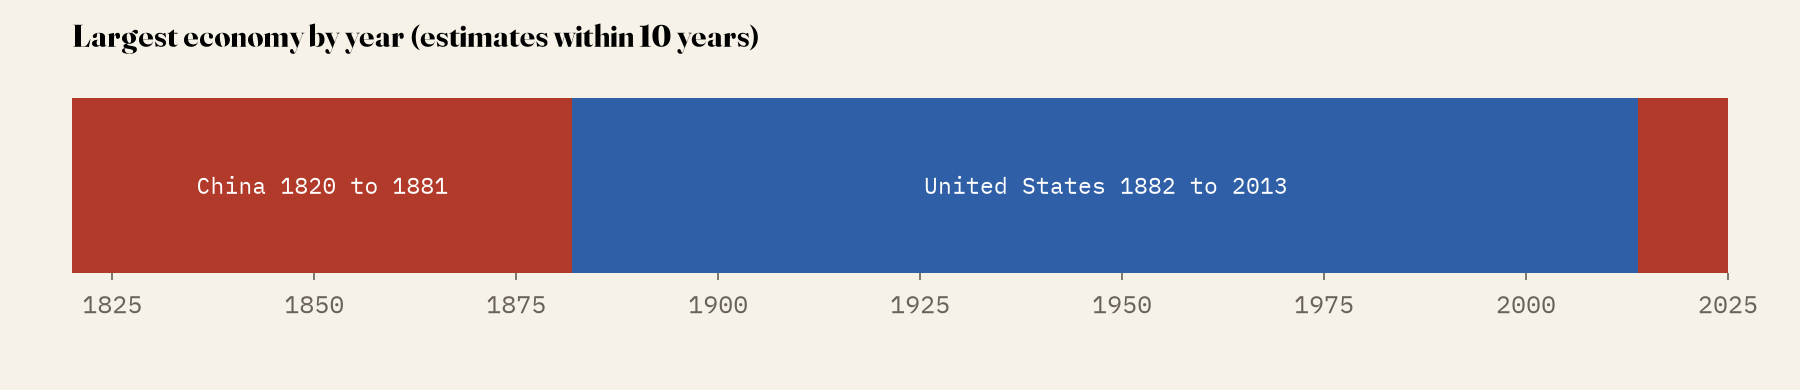
\includegraphics[width=\textwidth]{f_lead.png}
\caption{The largest economy in each year, using estimates within ten years.}\label{fig:lead}\end{figure}

\begin{table}[tbp]\centering\small\caption{Crossings: the first year in which one country's value exceeded another's, and the first year from which it stayed ahead to 2024 (none: fell behind again), judged on years in which both have their own estimate.}\label{tab:over}\begin{tabular}{llrrr}\toprule Crossing & Measure & First & Ahead since & Years compared\\\midrule
United States passes United Kingdom & GDP & 1862 & 1862 & 205\\
United States passes United Kingdom & GDP per head & 1880 & 1935 & 228\\
United States passes China & GDP & 1887 & none & 95\\
China passes United States (since 1950) & GDP & 2014 & 2014 & 75\\
India passes United Kingdom (since 1900) & GDP & 1921 & 1984 & 125\\
India passes Japan (since 1950) & GDP & 1950 & 2008 & 75\\
Japan passes United Kingdom & GDP per head & 1980 & 2023 & 154\\
South Korea passes Japan & GDP per head & 2019 & 2019 & 114\\
South Korea passes United Kingdom & GDP per head & 2020 & 2020 & 114\\
\bottomrule\end{tabular}\end{table}

\subsection{Take-offs}
Figure~\ref{fig:pc} shows GDP per head for six countries since 1870. Japan's was \$3,062 in 1950, 28\% of the British level, and \$18,226 in 1973, 95\% of it: a 6.0-fold rise at 8.1\% a year. Japan first passed the United Kingdom in 1980. South Korea's GDP per head was \$998 in 1950 and \$1,548 in 1960, 24\% of Japan's and below Ghana's (\$2,197); 88 of 122 countries of a million people or more were richer. It grew at 7.0\% a year from 1960 to 2000, passed Japan in 2019 and the United Kingdom in 2020, and reached \$42,751 in 2024, 28 times its 1960 level. China's GDP per head rose from \$1,744 in 1978 to \$21,339 in 2024 (12.2 times, 5.6\% a year).

Table~\ref{tab:fast} ranks countries of ten million people or more by their best 25-year growth of GDP per head since 1950. The first two, Iraq from 1991 and Angola from 1986, start from wartime collapses and are oil economies; the next three are South Korea, Japan and Taiwan, and China is eighth.

\begin{figure}[tbp]\centering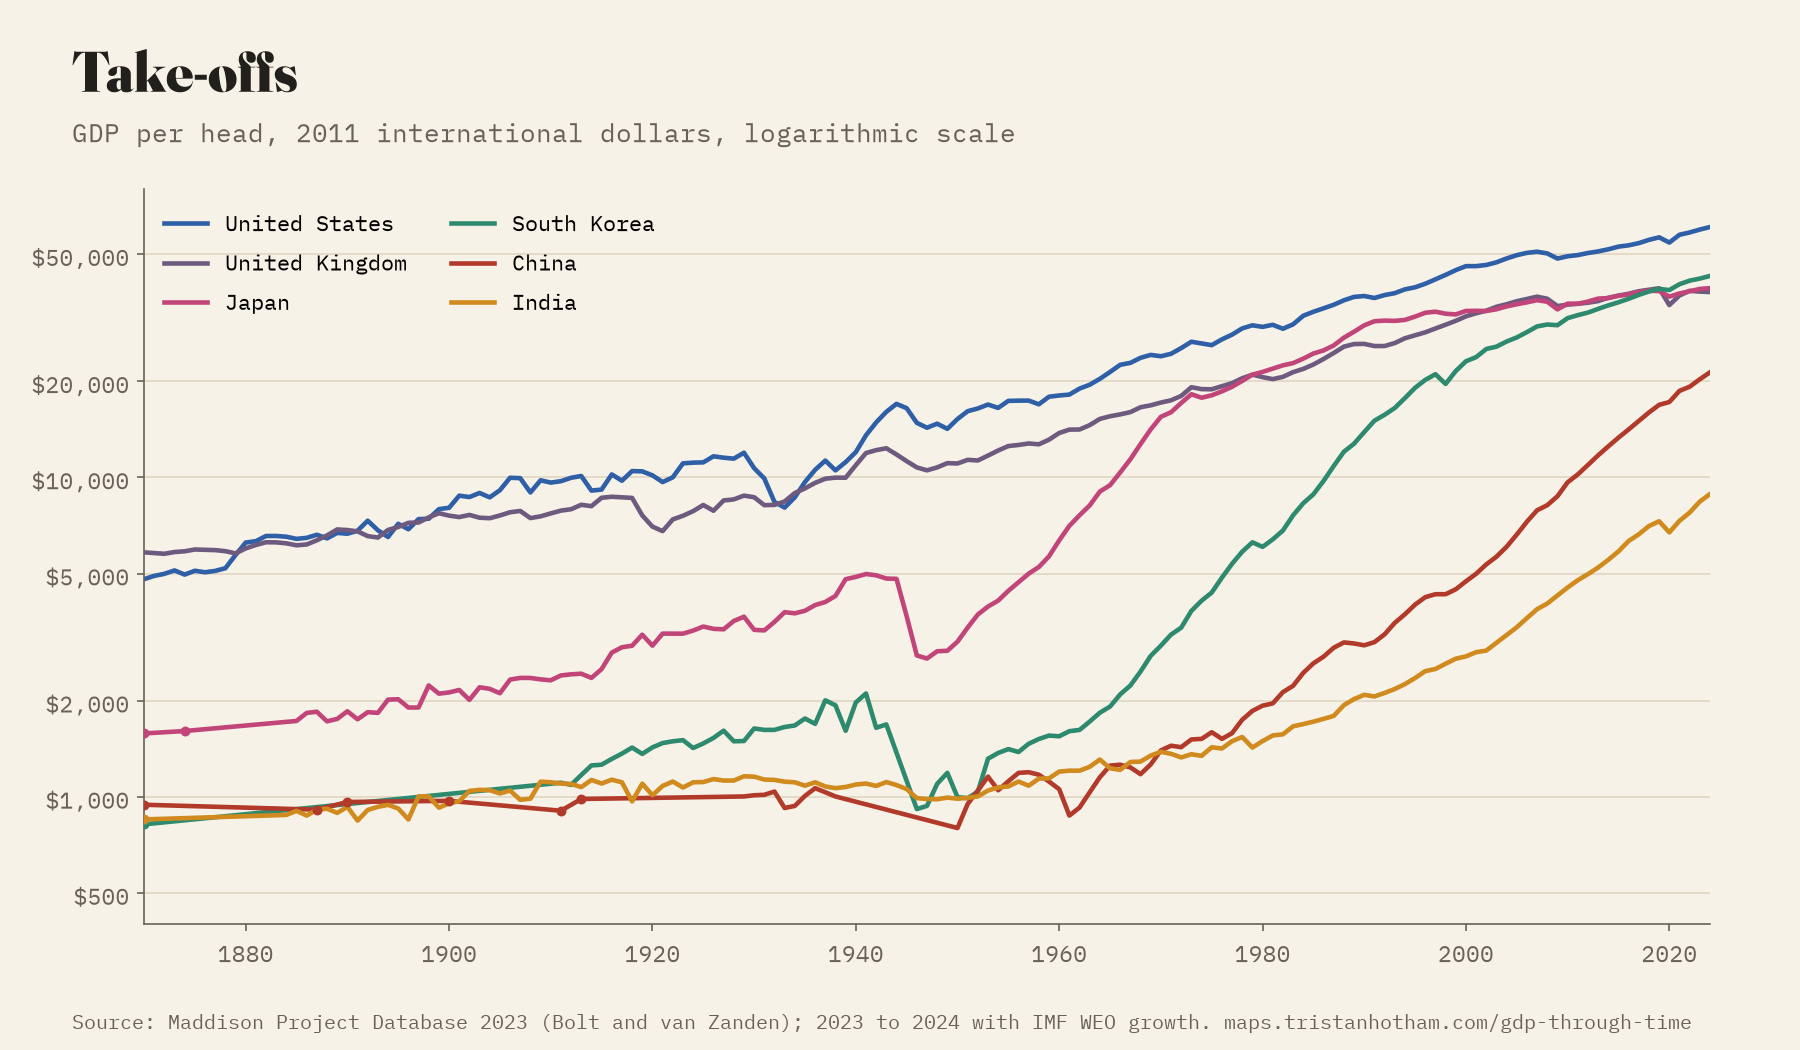
\includegraphics[width=\textwidth]{f_pc.png}
\caption{GDP per head, 1870 to 2024, 2011 international dollars, logarithmic scale.}\label{fig:pc}\end{figure}

\begin{table}[tbp]\centering\small\caption{Best 25-year growth of GDP per head since 1950, countries of ten million people or more (one spell per country).}\label{tab:fast}\begin{tabular}{lrrr}\toprule Country & Years & Growth (\% a year) & Multiple\\\midrule
Iraq & 1991 to 2016 & 9.3 & 9.3\\
Angola & 1986 to 2011 & 8.2 & 7.2\\
South Korea & 1965 to 1990 & 8.2 & 7.2\\
Japan & 1950 to 1975 & 7.4 & 5.9\\
Taiwan & 1962 to 1987 & 7.4 & 5.9\\
Romania & 1992 to 2017 & 6.5 & 4.8\\
Afghanistan & 1994 to 2019 & 6.4 & 4.7\\
China & 1992 to 2017 & 6.3 & 4.7\\
Myanmar & 1994 to 2019 & 6.2 & 4.5\\
Saudi Arabia & 1956 to 1981 & 6.1 & 4.4\\
\bottomrule\end{tabular}\end{table}

\subsection{The gap between rich and poor countries}
Among countries of a million people or more with their own estimate, the richest had 5.2 times the GDP per head of the poorest in 1820 (United Kingdom and Nepal), 9.1 in 1870, 11.6 in 1913, 29.5 in 1950, 130.5 in 2000 and 251.4 in 2024 (Qatar and the Central African Republic) (Table~\ref{tab:gap}, Figure~\ref{fig:gap}). Because the maximum is often a small oil exporter, the ratio of the 90th to the 10th percentile is a steadier measure: 3.0 in 1820, 6.0 in 1913, 10.6 in 1950, 28.1 in 2000 and 26.3 in 2024. Coverage changes are part of this: the number of such countries with estimates rises from 41 in 1820 to 150 in 2024, and the poorest are least likely to have early estimates, which biases early ratios down. The jump in 1950 in Figure~\ref{fig:gap} is mostly this effect.

Before 1820 the comparisons rest on very few countries. Among those with estimates, the Netherlands was the richest in 1600 and 1700 (\$3,377 in 1700; Table~\ref{tab:pre}); the second in 1700 is ``South Africa'', which in this database means the Dutch settler colony at the Cape, a small part of today's territory.

\begin{figure}[tbp]\centering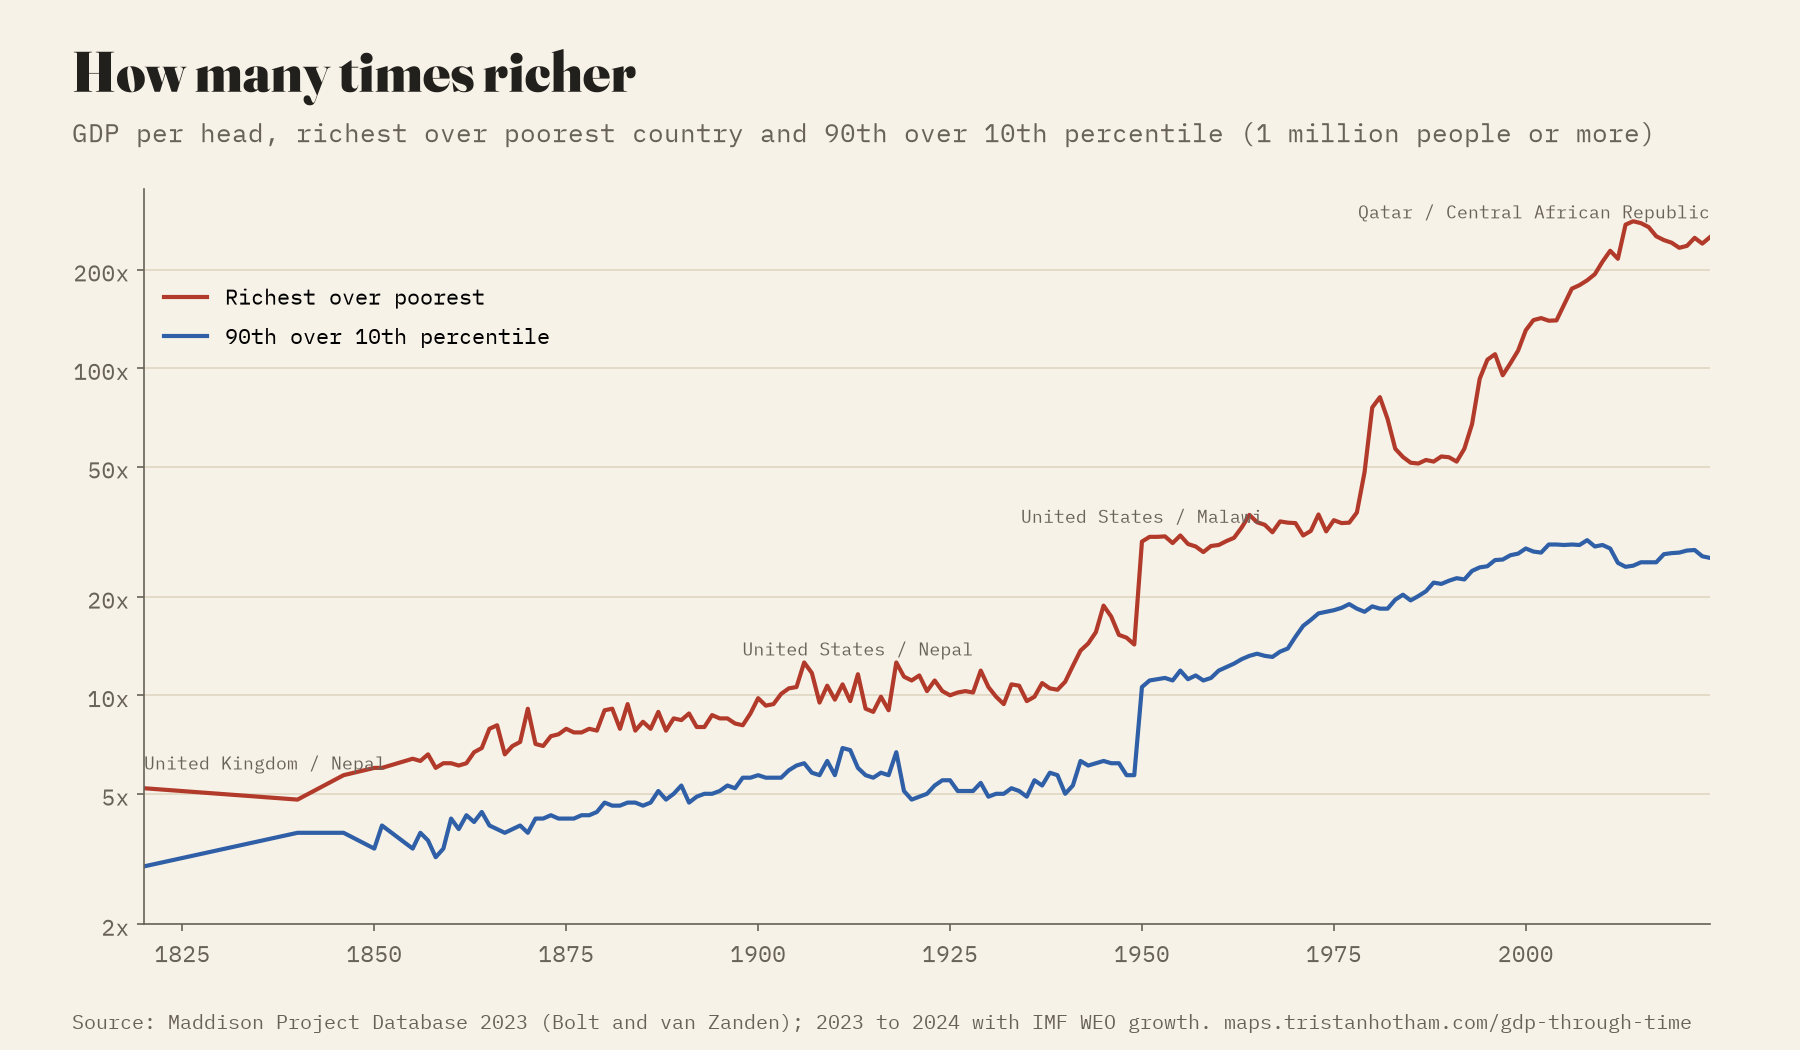
\includegraphics[width=\textwidth]{f_gap.png}
\caption{Ratio of the highest to the lowest, and of the 90th to the 10th percentile, GDP per head among countries of a million people or more with their own estimate (years with at least 20 such countries).}\label{fig:gap}\end{figure}

\begin{table}[tbp]\centering\small\caption{Richest and poorest countries by GDP per head (2011 int.\ \$), countries of a million people or more with their own estimate.}\label{tab:gap}\begin{tabular}{rrlrlrrr}\toprule Year & Countries & Richest & & Poorest & & Ratio & p90/p10\\\midrule
1500 & 9 & Belgium & 2,338 & Turkey & 768 & 3.0 & 2.1\\
1600 & 13 & Netherlands & 4,270 & Mexico & 799 & 5.3 & 2.5\\
1700 & 16 & Netherlands & 3,377 & Turkey & 897 & 3.8 & 2.5\\
1820 & 41 & UK & 3,306 & Nepal & 641 & 5.2 & 3.0\\
1870 & 57 & UK & 5,829 & Nepal & 641 & 9.1 & 3.8\\
1913 & 60 & US & 10,108 & Nepal & 870 & 11.6 & 6.0\\
1950 & 111 & US & 15,240 & Malawi & 516 & 29.5 & 10.6\\
1973 & 119 & US & 26,602 & Chad & 746 & 35.7 & 17.8\\
2000 & 150 & Norway & 54,040 & DR Congo & 414 & 130.5 & 28.1\\
2022 & 153 & Qatar & 149,171 & Central African Rep. & 596 & 250.1 & 27.8\\
2024 & 150 & Qatar & 146,965 & Central African Rep. & 585 & 251.4 & 26.3\\
\bottomrule\end{tabular}\end{table}

\begin{table}[tbp]\centering\small\caption{Highest GDP per head (2011 int.\ \$) among countries of a million people or more with an estimate within ten years, 1700, 1820 and 1913.}\label{tab:pre}\begin{tabular}{lrlrlr}\toprule \multicolumn{2}{c}{1700} & \multicolumn{2}{c}{1820} & \multicolumn{2}{c}{1913}\\\midrule
Netherlands & 3,377 & United Kingdom & 3,306 & United States & 10,108\\
South Africa & 2,715 & Netherlands & 3,006 & Australia & 8,220\\
United Kingdom & 2,412 & United States & 2,674 & United Kingdom & 8,212\\
Belgium & 2,192 & Italy & 2,523 & New Zealand & 8,212\\
Sweden & 2,002 & Belgium & 2,358 & Switzerland & 8,172\\
France & 1,758 & Germany & 2,041 & Canada & 7,088\\
Portugal & 1,572 & Denmark & 2,031 & Belgium & 6,727\\
China & 1,543 & Austria & 1,941 & Netherlands & 6,454\\
Germany & 1,511 & France & 1,809 & Denmark & 6,236\\
Mexico & 1,476 & Portugal & 1,665 & Argentina & 6,052\\
\bottomrule\end{tabular}\end{table}

\begin{figure}[tbp]\centering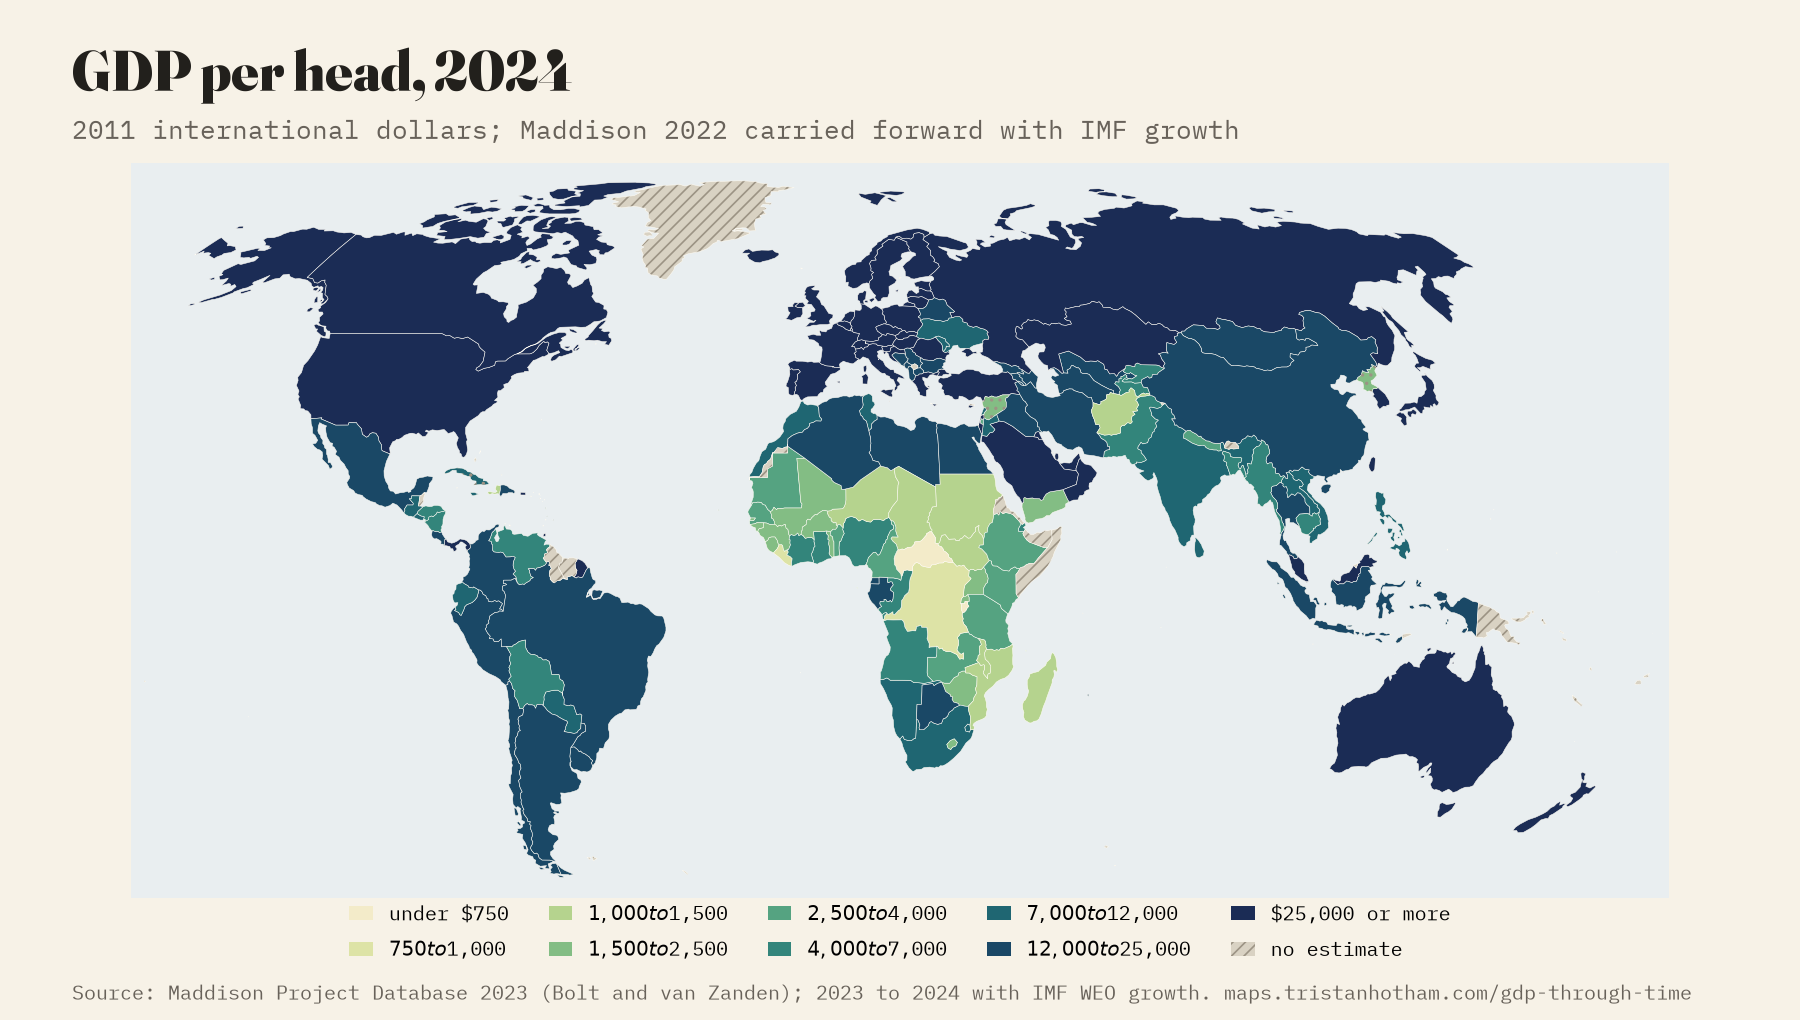
\includegraphics[width=\textwidth]{f_pcmap.png}
\caption{GDP per head in 2024 (2022 values carried forward with IMF growth).}\label{fig:pcmap}\end{figure}

\section{Limitations}\label{sec:limits}
The figures are estimates built on very different evidence. Before AD 1 the world series are reconstructions that assume output per head near subsistence and infer population from archaeology and carrying capacity; the two population series used here differ by a factor of two to three in the third millennium BC, and HYDE's own range is wider still. Before 1820, and for much of Africa, the Middle East and Asia before 1950, they rest on wages, prices, harvest and tax records, and on assumptions about population; for AD 1 several countries share a single regional value. Purchasing power comparisons across two centuries depend on one set of 2011 prices and on the volume growth of each country's own accounts, so levels in the distant past carry wide margins. GDP measures market production, not well-being, and says nothing about its distribution within countries.

Present-day borders are a choice of the database, not of history: the colours describe modern territories, and the borders of the time are only a backdrop. Former states are shown whole until they broke up, but their successors' own series exist for earlier years and appear in the country charts. World totals before 1950 depend on the database's regional estimates for countries without their own series, and shares between benchmark years use an interpolated total. The extension to 2024 uses another institution's growth rates on a different PPP basis (ICP 2021), and some of the IMF's latest figures are estimates. The ``nearest estimate'' filling on the map can make a sparse record look fuller than it is; it can be switched off. Finally, releases of the database revise past values, sometimes by large amounts, and all results should be read as describing the 2023 release.

\section{Conclusion}
On one map, two centuries of the world economy show a clear arc: dominance by the populous economies of Asia, a long Western ascendancy that peaked before the First World War, and a return of China and India to a combined third of world output, achieved through some of the fastest sustained growth ever recorded. The same map shows how little of the earlier past the evidence covers. The data, code and interactive version are published so the numbers can be checked and updated with each new release.

\section*{Data and code availability}
The interactive version is at \url{https://maps.tristanhotham.com/gdp-through-time/}. Data and code are at \url{https://github.com/Tristan-Hotham/gdp-through-time} and archived with this paper at https://doi.org/10.5281/zenodo.23899403. Derived data are released under CC BY 4.0 (the Maddison Project Database is CC BY 4.0) and code under the MIT licence; the simplified historical borders keep the GPL-3.0 licence of historical-basemaps.

\section*{AI statement}
I wrote the text, with drafting and editing assistance from Claude (Anthropic), which also helped prepare the analysis code. I reviewed and checked all text and results.

\appendix
\section{Sources of the series shown}
The Maddison Project asks that the original studies be cited when fewer than twelve countries are shown. Table~\ref{tab:src} lists, from the database's own sources sheet, the main sources of the long series for the countries drawn individually in the figures.

\begin{longtable}{lp{2.2cm}p{11cm}}\caption{Sources of the long series for the countries shown, as listed in the Maddison Project Database 2023 sources sheet (recent years: national accounts and the Conference Board Total Economy Database).}\label{tab:src}\\\toprule Code & Years & Source\\\midrule\endhead
CHN & 1000-1661 & Broadberry, S.N., Guan, Hanhui and David Daokui Li (2018), ''China, Europe and the Great Divergence: a Study in Historical National Accounting, 980-1850'', Journal of Economic History, 78, 4, 955-1000\\
CHN & 1661 to 1933 & Xu, Y. Z. Shi, B. van Leeuwen, Y Ni, Z Zhang, and Y Ma, (2016) 'Chinese National Income, ca. 1661-1933', Australian Economic History Review 57(3), 368 to 393\\
CHN & 1952 to 2008 & Wu, Harry X. (2014), ''China's growth and productivity performance debate revisited, Accounting for China's sources of growth with a new data set'' The Conference Board Economics Program Working Paper Series EWP\#14-01.\\
IND & 1600 to 1870 & Broadberry, S.N., Custodis, J. and Gupta, B. (2015), ''India and the great divergence: an Anglo-Indian comparison of GDP per capita, 1600 to 1871'' Explorations in Economic History, 55: 58-75.\\
USA & 1650 - 1790 & McCusker, John J., 'Colonial Statistics', Historical Statistics of the United States: Earliest Time to the Present, in S. B. Carter, S. S. Gartner, M. R. Haineset al. New York, Cambridge University Press. V-671.\\
USA & 1790 - 1870 & Sutch, R. (2006). National Income and Product. Historical Statistics of the United States: Earliest Time to the Present, in S. B. Carter, S. S. Gartner, M. R. Haineset al. New York, Cambridge University Press III-23-25.\\
USA & 1800-1830 & Prados de la Escosura, L. (2009). ''Lost Decades? Economic Performance in Post-Independence Latin America,'' Journal of Latin America Studies 41: 279 to 307. (updated data)\\
GBR & 1 & Scheidel, W. and Friesen, S. J., 'The size of the economy and the distribution of income in the Roman Empire', Journal of Roman Studies, 99 (2009), pp. 61 to 91\\
GBR & 1252 to 1700 (England) & Broadberry, S.N., B. Campbell, A. Klein, M. Overton and B. van Leeuwen (2015), British Economic Growth 1270-1870 Cambridge: Cambridge University Press.\\
JPN & 724-1874 & Bassino, Jean-Pascal \& Broadberry, Stephen \& Fukao, Kyoji \& Gupta, Bishnupriya \& Takashima, Masanori, (2018). ''Japan and the Great Divergence, 730-1874,'' CEI Working Paper Series 2018-13, Center for Economic Institutions, Institute of Economic Research, Hitotsubashi University\\
JPN & 1874-1940 & Fukao, K., Bassino, J.-P., Makino, T., Paprzycki, R., Settsu, T., Takashima, M., and Tokui, J. (2015) Regional Inequality and Industrial Structure in Japan: 1874-2008, Tokyo: Maruzen Publishing.\\
KOR & 1911-1990 & Cha, M.S., Kim, N.N., Park, K.-J., Park, Y. (Eds.) (2020), Historical Statistics of Korea. Studies in Economic History, New York: Springer Publishing\\
DEU & 1500-1850 & Pfister, U. (2022). Economic Growth in Germany, 1500 to 1850. The Journal of Economic History, 82(4), 1071 to 1107\\
NLD & 1348 to 1807 (Holland) & Van Zanden, J. L. and van Leeuwen, B. (2012), 'Persistent but not consistent: the growth of national income in Holland 1347 to 1807', Explorations in Economic History, 49 (2012), pp. 119 to 30.\\
NLD & 1807-1913 & Smits, J.P., E. Horlings and J.L. van Zanden (2000). The Measurement of Gross National Product and its Components 1800-1913 (Groningen Growth and Development Centre Monograph series no 5).\\
\bottomrule\end{longtable}

\begin{thebibliography}{20}
\bibitem[Bassino et~al.(2019)]{bassino2019} Bassino, J.-P., Broadberry, S., Fukao, K., Gupta, B. and Takashima, M. (2019) Japan and the great divergence, 730 to 1874. \textit{Explorations in Economic History}, 72, 1 to 22.
\bibitem[Bolt and van Zanden(2024)]{mpd2023} Bolt, J. and van Zanden, J. L. (2024) Maddison style estimates of the evolution of the world economy: a new 2023 update. \textit{Journal of Economic Surveys}. Data: Maddison Project Database, version 2023, DataverseNL, \url{https://doi.org/10.34894/INZBF2}. CC BY 4.0.
\bibitem[Broadberry et~al.(2015a)]{broadberry2015} Broadberry, S., Campbell, B. M. S., Klein, A., Overton, M. and van Leeuwen, B. (2015) \textit{British Economic Growth, 1270 to 1870}. Cambridge University Press.
\bibitem[Broadberry et~al.(2015b)]{broadberry2015india} Broadberry, S., Custodis, J. and Gupta, B. (2015) India and the great divergence: an Anglo-Indian comparison of GDP per capita, 1600 to 1871. \textit{Explorations in Economic History}, 55, 58 to 75.
\bibitem[Broadberry et~al.(2018)]{broadberry2018} Broadberry, S., Guan, H. and Li, D. D. (2018) China, Europe and the great divergence: a study in historical national accounting, 980 to 1850. \textit{Journal of Economic History}, 78(4), 955 to 1000.
\bibitem[IMF(2025)]{weo2025} International Monetary Fund (2025) World Economic Outlook database, October 2025. \url{https://www.imf.org/en/Publications/WEO}
\bibitem[De Long(1998)]{delong1998} De Long, J. B. (1998) Estimates of world GDP, one million B.C. to present. Working paper, University of California, Berkeley.
\bibitem[Klein Goldewijk et~al.(2017)]{hyde2017} Klein Goldewijk, K., Beusen, A., Doelman, J. and Stehfest, E. (2017) Anthropogenic land use estimates for the Holocene: HYDE 3.2. \textit{Earth System Science Data}, 9, 927 to 953.
\bibitem[Maddison(2010)]{maddison2010} Maddison, A. (2010) Historical Statistics of the World Economy: 1 to 2008 AD. Groningen Growth and Development Centre.
\bibitem[McEvedy and Jones(1978)]{mcevedy1978} McEvedy, C. and Jones, R. (1978) \textit{Atlas of World Population History}. Penguin.
\bibitem[Roodman(2020)]{roodman2020} Roodman, D. (2020) Modeling the human trajectory. Open Philanthropy. Data and code: \url{https://github.com/droodman/Modeling-Human-Trajectory}
\bibitem[Maddison(2001)]{maddison2001} Maddison, A. (2001) \textit{The World Economy: A Millennial Perspective}. OECD Development Centre.
\bibitem[Maddison(2007)]{maddison2007} Maddison, A. (2007) \textit{Contours of the World Economy, 1 to 2030 AD}. Oxford University Press.
\bibitem[Natural Earth(2026)]{naturalearth} Natural Earth (2026) Admin 0 countries, 1:50m. Public domain. \url{https://www.naturalearthdata.com/}
\bibitem[Ourednik(2026)]{ourednik} Ourednik, A. and contributors (2026) historical-basemaps: historical boundaries of world countries and cultural regions. GPL-3.0. \url{https://github.com/aourednik/historical-basemaps}
\bibitem[Pomeranz(2000)]{pomeranz2000} Pomeranz, K. (2000) \textit{The Great Divergence: China, Europe, and the Making of the Modern World Economy}. Princeton University Press.
\bibitem[Scheidel and Friesen(2009)]{scheidel2009} Scheidel, W. and Friesen, S. J. (2009) The size of the economy and the distribution of income in the Roman Empire. \textit{Journal of Roman Studies}, 99, 61 to 91.
\end{thebibliography}
\end{document}
